\section{Ergänzende Instrumente}

\textbf{Anhang der Kapitalgesellschaft}:
\begin{itemize}
	\item \textbf{Erläuterungs-}, \textbf{Ergänzungs-}, \textbf{Entlastungs-} (Verlagerung von Informationen in den Anhang), \textbf{Korrekturfunktion} (Angaben zur Vermeidung von Fehlinformation) für Bilanz und GuV
	\item Zwei Arten von Angaben im Anhang:
	\begin{itemize}
		\item \textbf{Pflichtangaben}:
		\begin{itemize}
			\item Angaben, die immer im Anhang zu machen sind
			\item Angaben, die aufgrund der eines Wahlrechts nicht in Bilanz oder GuV aufgenommen wurden
			\item Bilanzierungs- und Bewertungsmethoden, die auf Bilanz und GuV angewendet wurden
			\item Abweichungen von Bilanzierungs- und Bewertungsmethoden
			\item Unterschiedsbeträge
			\item Einbeziehung von Fremdkapitalzinsen in die Herstellungskosten
			\item Darstellung des Anlagevermögens mit Hilfe eines \textbf{Anlagespiegels}
			\begin{center}
				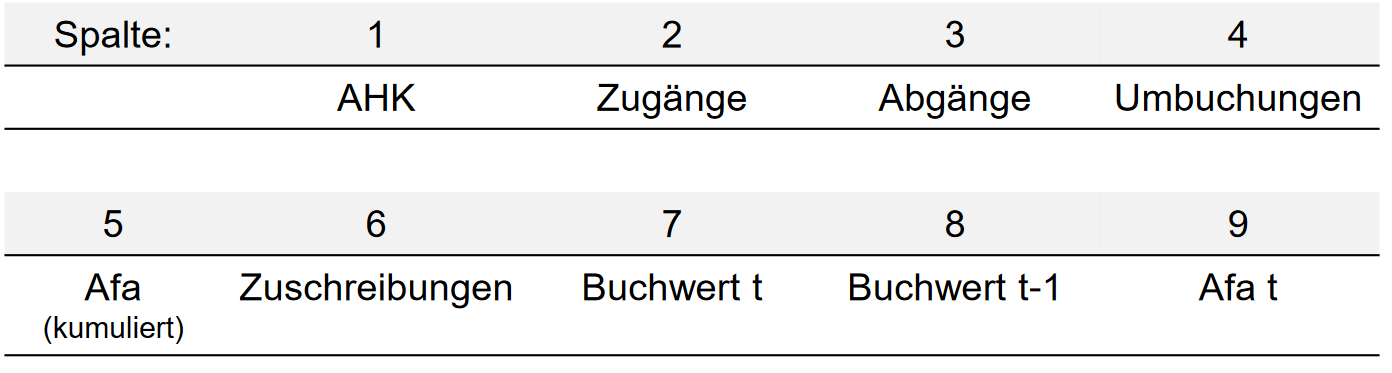
\includegraphics[width=0.7\textwidth]{images/anmirr.png}
			\end{center}
			$\rightarrow$ Darlegung von im Anlagevermögen gebundene Kapital, Altersstruktur der Vermögensgegenstände und der Entwicklung der einzelnen Posten.
		\end{itemize}
		\item \textbf{Sonstige Pflichtangaben}: 
		\begin{itemize}
			\item Fristigkeit und Besicherung der Verbindlichkeiten
			\item Informationen zu außerbilanziellen Geschäften
			\item Gesamtbeträge sonstiger finanzieller Verpflichtungen
			\item Aufgliederung der Umsatzerlöse
			\item Weitere Inhalte s. FS6/12-14
		\end{itemize}
	\end{itemize}
\end{itemize}

\textbf{Unterlassen von Angaben}:
\begin{itemize}
	\item Zwingende Unterlassung von Angaben mit Rücksicht auf das Wohl des Landes
	\item Unerhebliche Beteiligungen können unterlassen werden
	\item Aufgliederung der Umsatzerlöse kann unterbleiben, wenn KapG dadurch Nachteil erleidet
	\item Erleichterungen für kleine und mittelgroße KapG
\end{itemize}
\bigskip
\textbf{Lagebericht der Kapitalgesellschaft}:
\begin{itemize}
	\item Pflicht für große und mittelgroße KapG, kleine KapG befreit
	\item Eigenständiges Informationsinstrument mit Rechenschafts- und Informationsfunktion, das Vorgaben genügt und geprüft werden muss.
\end{itemize}

\textbf{Inhalt des Lageberichts}:
\begin{itemize}
	\item Geschäftsverlauf den tatsächlichen Verhältnissen entsprechend darstellen
	\item Bedeutsamen finanzielle Leistungsindikatoren einbeziehen
	\item Zukünftige Entwicklung beurteilen
	\item Große Kap: Eingehen auf \textbf{nicht-finanzielle Leistungsindikatoren} (z.B. Kundenzufriedenheit)
	\item Kapitalmarktorientierte KapG müssen Merkmale des internen Kontroll- und des Risikomanagementsystems beschreiben
	\item Weitere Inhalte s. FS6/21,23-26
\end{itemize}

\textbf{Nichtfinanzielle Berichterstattung}:
\begin{center}
	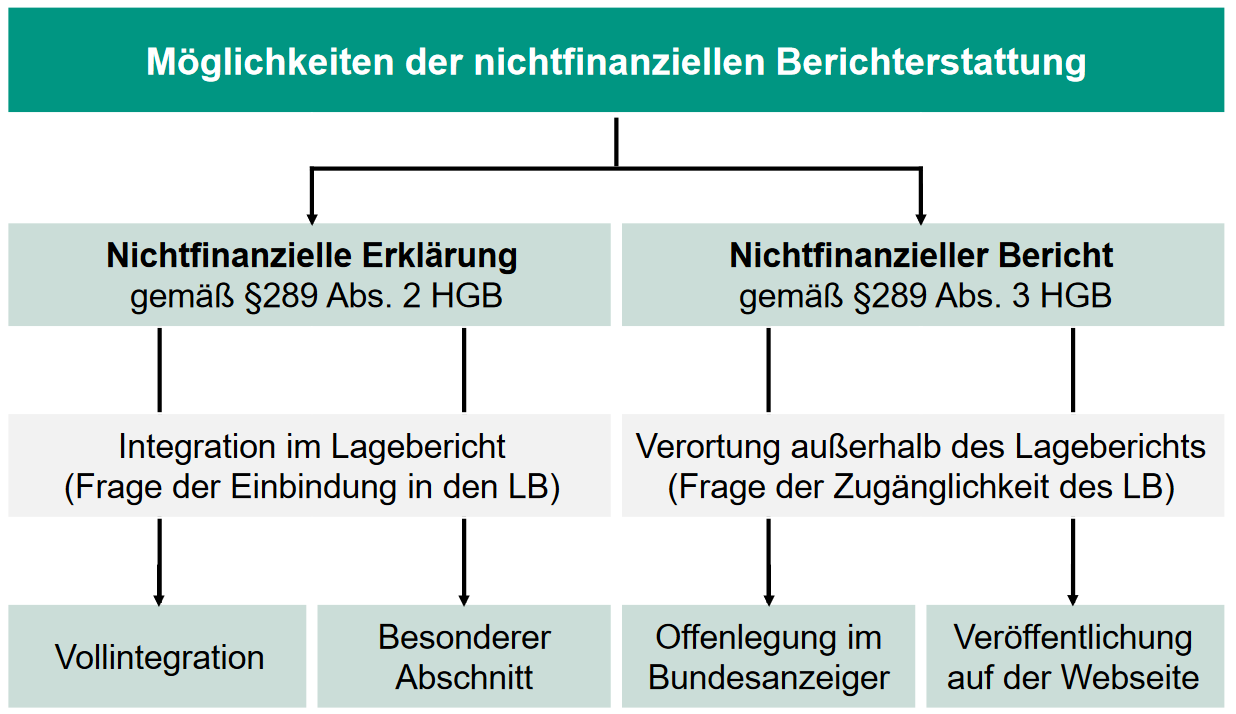
\includegraphics[width=0.6\textwidth]{images/nfb.png}
\end{center}
\textbf{Muss folgende Aspekte beinhalten}: Umweltbelange, Arbeitnehmerbelange, Sozialbelange, Achtung der Menschenrechte, Bekämpfung von Korruption und Bestechung\\
 
\textbf{Kapitalflussrechnung}: 
\begin{itemize}
	\item Informiert über Herkunft und Verwendung der finanziellen Mittel eines Unternehmens
	\item Ergänzungsrechnung zum JA zur Schließung der finanzwirtschaftlichen Informationslücke
	\item Pflicht für kapitalmarktorientierte KapG, freiwillig für Einzelunternehmen
	\item KFR ist eine \textbf{Zeitraumrechnung}
	\item \textbf{DRS 21} als Leitlinie zur Aufstellung einer KFR
\end{itemize}

\textbf{Kapitalflussrechnung nach DRS 21}:
\begin{itemize}
	\item Enthält Mindestgliederung
	\item Darstellung getrennt nach den betrieblichen Funktionsbereichen: Laufende Geschäftstätigkeit, Investitionstätigkeit, Finanzierungstätigkeit in \textbf{Staffelform}
	\item \textbf{Derivative Ermittlung} aus den Daten des externen Rechnungswesen:
	\begin{itemize}
		\item \textbf{Direkte Ermittlung}: Aufwendungen und Erträge werden um nicht zahlungswirksame Bestandteile korrigiert
		\item \textbf{Indirekte Ermittlung}: Periodenergebnis wird um nicht zahlungswirksame Aufwendungen und Erträge korrigiert, und um zahlungswirksame Veränderungen des Nettoumlaufvermögens ergänzt.
	\end{itemize}
	Gliederungsschema s.FS6/33-37
\end{itemize}

\textbf{Zusammenhang von KFR, Bilanz und GuV}:
\begin{center}
	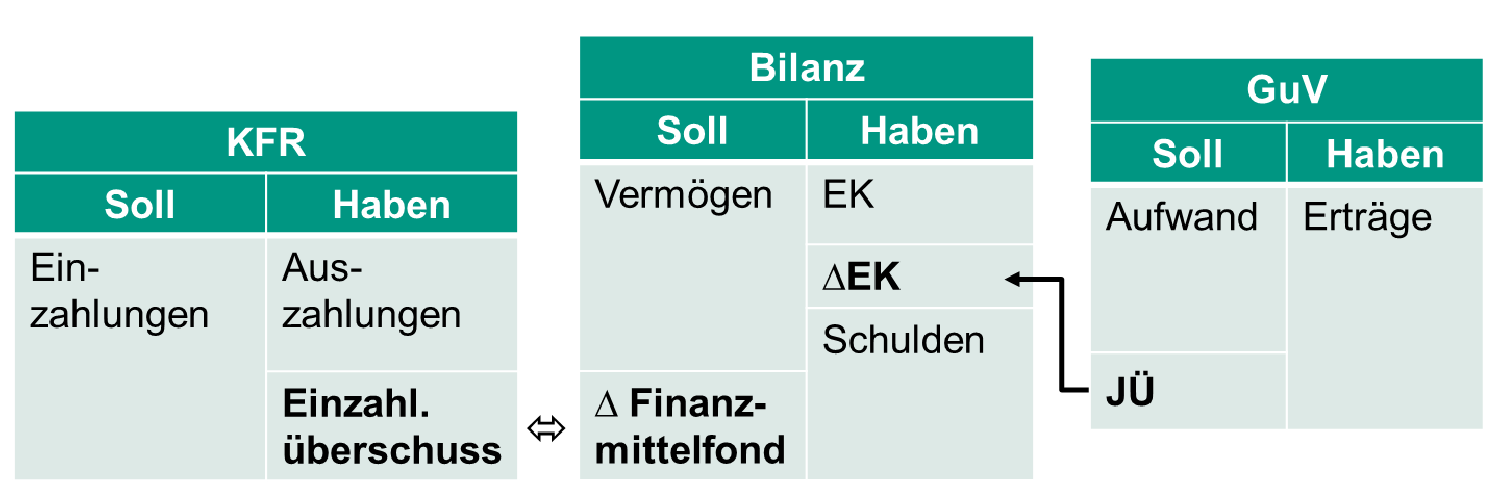
\includegraphics[width=0.8\textwidth]{images/kbg.png}
\end{center}

\textbf{Eigenkapitalspiegel}: Darstellung der Eigenkapitalveränderungen während einer Rechnungsperiode
\begin{itemize}
	\item Pflicht nur für kapitalmarktorientierte KapG
	\item Darstellung orientiert sich am \textbf{DRS 7} mit Inhalt:
	\begin{itemize}
		\item Aufschlüsselung der EK-Positionen
		\item Anfangs- und Endbestände der EK-Positionen
		\item Ereignisse, welche die EK-Positionen verändert haben
	\end{itemize}
	$\rightarrow$ Verwendung des JÜ wird sichtbar gemacht
\end{itemize}

\textbf{Segmentberichterstattung}: Informationen über die wesentlichen Geschäftsbereiche eines Unternehmens
\begin{itemize}
	\item Freiwillig und inhaltlich durch \textbf{DRS 3} konkretisiert
	\item \textbf{Segment}: Teil eines Unternehmens, das (potentiell) Umsatzerlöse erzielt und
	das regelmäßig von der Geschäftsleitung zur Beurteilung der wirtschaftlichen Lage überwacht wird
	\item Unterscheide \textbf{produktorientierte} und \textbf{geographische} Segmente
	\item \textbf{Pflichtangaben je Segment}: Segmentumsatzerlöse, Segmentergebnis, Sonstige Angaben (z.B. Segmentvermögen und Segmentschulden)
\end{itemize}

\textbf{Übersicht: Umfang der handelsrechtlichen Finanzberichterstattung}
\begin{center}
	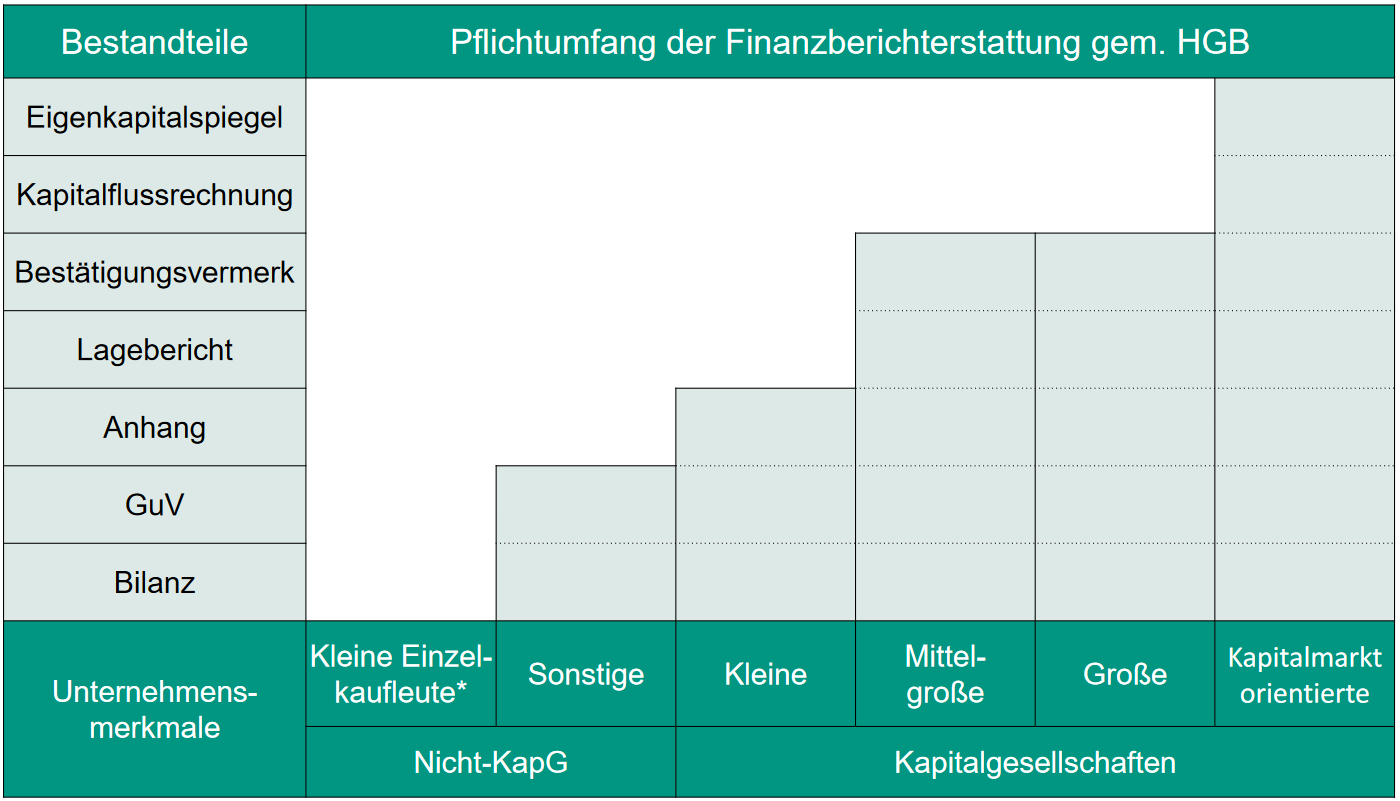
\includegraphics[width=0.8\textwidth]{images/sum.png}
\end{center}